\documentclass[10pt,a4paper]{report}

\usepackage{amsmath}
\usepackage{amsfonts}
\usepackage{amssymb}
\usepackage{hyperref}
\usepackage{url}
\usepackage{multirow}
\usepackage{graphicx}

\author{Barbara Bruno}
\title{HMP-Detector Documentation}

\begin{document}
\maketitle

\tableofcontents

\chapter{Preliminary Info}
\section{Contact Info}

\textbf{Barbara Bruno} (Ph.D. student)\\
Laboratorium @ DIBRIS\\
Department of Computer Science, Bioengineering, Robotics and Systems Engineering\\
University of Genova, Italy\\
Via all'Opera Pia 13, 16145, Genova, Italy\\
\url{barbara.bruno@unige.it}

\section{References}

The \textbf{docs} folder provided with this distribution contains:
\begin{itemize}
\item an introductory PowerPoint presentation providing an overview of the system (ppsx format: it requires Microsoft PowerPoint Viewer);
\item this user guide.
\end{itemize}
Detailed information about the system can be found at:
\begin{itemize}
\item Bruno, B., Mastrogiovanni, F., Sgorbissa, A., Vernazza, T., Zaccaria, R.: Human motion modelling and recognition: A computational approach. In: IEEE Int Conf on Automation Science and Engineering (CASE), pp. 156--161 (2012)
\item Bruno, B., Mastrogiovanni, F., Sgorbissa, A., Vernazza, T., Zaccaria, R.: Analysis of human behavior recognition algorithms based on acceleration data. In: IEEE Int Conf on Robotics and Automation (ICRA), pp. 1602--1607 (2013)
\end{itemize}

\chapter{System Requirements}
\section{OS Requirements}

The system has been tested under:
\begin{itemize}
\item Ubuntu 11.10:\\
free download at \url{http://releases.ubuntu.com/11.10/} 
\item Ubuntu 12.04.2 LTS:\\
free download at \url{http://old-releases.ubuntu.com/releases/precise/}
\end{itemize}
\textbf{Installation instructions in this guide refer to Ubuntu 12.04.2 OS.}

\section{Hardware Requirements}

The HMPdetector allows for both off-line and on-line analysis of accelerometer data for: (i) detection of Human Motion Primitives (HMP); (ii) detection of falls.

The on-line analysis requires the following three devices:
\begin{itemize}
\item \textbf{collector}, shown in Figure \ref{fig:collector}, to be connected to a USB port of the computer running the HMPdetector software;
\item \textbf{wrist device}, shown in Figure \ref{fig:wrist_device}, to be properly attached at the user right wrist;
\item \textbf{waist device}, shown in Figure \ref{fig:waist_device}, to be properly attached at the user belt.
\end{itemize}

The wrist device requires to be loaded with the Arduino function \verb+NonClassifier.ino+ that can be found inside folder \verb+./arduino/NonClassifier/+ inside the HMPdetector package.

The waist device requires to be loaded with the Arduino function \verb+FallDetector.ino+ that can be found inside folder \verb+./arduino/FallDetector/+ inside the HMPdetector package.

\begin{figure}
\centering
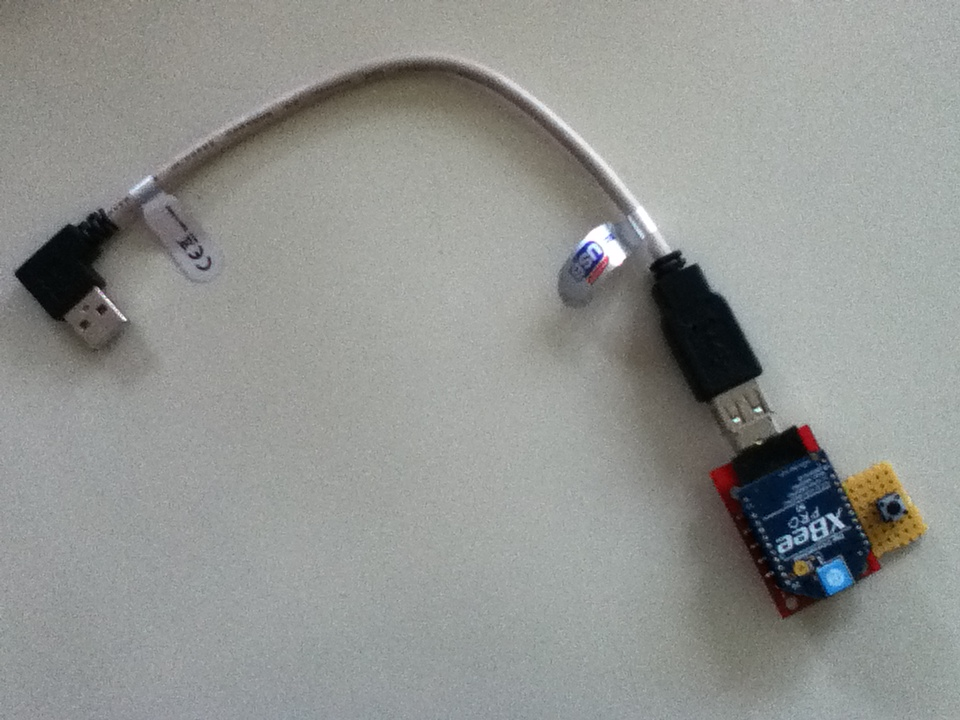
\includegraphics[scale=0.35]{HW_collector.jpg}
\caption{Collector device: for sensory data acquisition}
\label{fig:collector}
\end{figure}
\begin{figure}
\centering
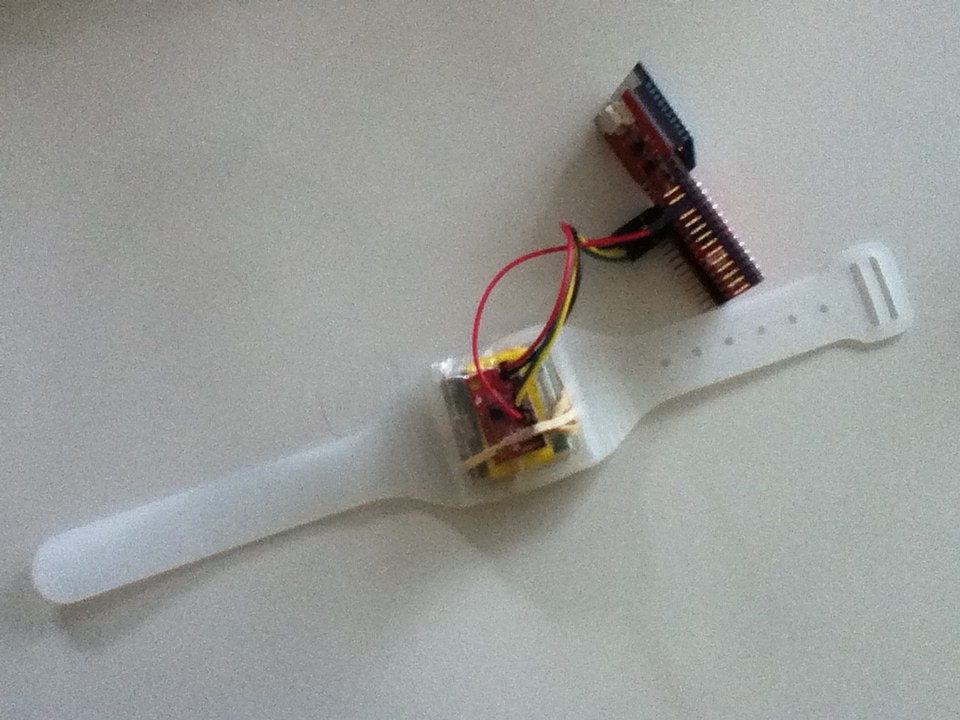
\includegraphics[scale=0.35]{HW_wrist_device.jpg}
\caption{Wrist-placed sensing device: for HMP detection}
\label{fig:wrist_device}
\end{figure}
\begin{figure}
\centering
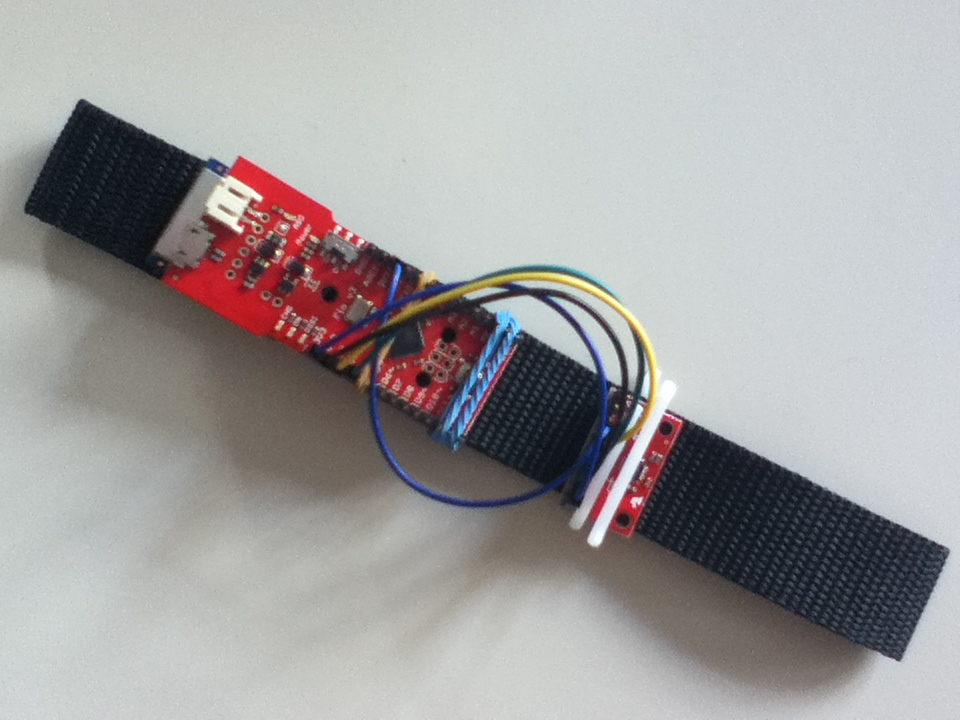
\includegraphics[scale=0.35]{HW_waist_device.jpg}
\caption{Waist-placed sensing device: for Fall detection}
\label{fig:waist_device}
\end{figure}

\chapter{Getting Started}
\section{Package description}

The HMPdetector package is provided with the following subfolders:
\begin{center}
\begin{tabular}{|c|c|c|}
\hline
\textbf{Name} & \textbf{Type} & \textbf{Description}\\
\hline
arduino & folder & Arduino middleware embedded on the sensing devices\\
\hline
docs & folder & HMPdetector documentation\\
\hline
libs & folder & C++ static libraries required by the HMPdetector software\\
\hline
Models & folder & Training datasets for all provided basic Human Motion Primitives\\
\hline
Results & folder & Output folder for all the debug/test functions\\
\hline
Validation & folder & Validation dataset for all provided basic Human Motion Primitives\\
\hline
\end{tabular}
\end{center}
and the following files:
\begin{center}
\begin{tabular}{|c|c|p{6cm}|}
\hline
\textbf{Name} & \textbf{Type} & \textbf{Description}\\
\hline
classifier.cpp & \multirow{2}{*}{C++ class} & \multirow{2}{*}{HMPdetector classifier module}\\
\cline{1-1}
classifier.hpp & & \\
\hline
CMakeLists.txt & CMake file & CMake build script\\
\hline
creator.cpp & \multirow{2}{*}{C++ class} & \multirow{2}{*}{HMPdetector models creator module}\\
\cline{1-1}
creator.hpp & & \\
\hline
FallDetector.cpp & \multirow{2}{*}{C++ class} & \multirow{2}{*}{Fall detector module}\\
\cline{1-1}
FallDetector.hpp & & \\
\hline
HMPdetector.cpp & C++ main & HMPdetector main\\
\hline
reasoner.cpp & \multirow{2}{*}{C++ class} & \multirow{2}{*}{HMPdetector reasoner module}\\
\cline{1-1}
reasoner.hpp & & \\
\hline
utils.cpp & \multirow{2}{*}{C++ methods} & \multirow{2}{*}{Frequently used functions}\\
\cline{1-1}
utils.hpp & & \\
\hline
viewPossibilities.m & MATLAB/Octave script & Visualization method for the HMPdetector classifier output\\
\hline
\end{tabular}
\end{center}

\section{Installation Guide}
\label{Installation Guide}
\subsection{Third-party libraries}

HMPdetector makes use of: (i) BOOST (collection of portable C++ source libraries), (ii) ARMADILLO (C++ linear algebra library), which requires LAPACK and BLAS libraries for optimal performance, and (iii) PEIS (middleware for Ambient Intelligence applications).

Detailed information about BOOST can be found at:\\
\url{http://www.boost.org/}

Detailed information about ARMADILLO can be found at:\\ \url{http://arma.sourceforge.net/}

Detailed information about PEIS can be found at:\\ \url{http://aass.oru.se/~peis/frameset_page.html}

The HMPdetector package comes with MATLAB/Octave scripts for graphical display of the system output. The download and installation instructions for both MATLAB (licensed) and Octave (free) are NOT included in this Installation Guide.

Detailed information about Octave can be found at:\\ \url{http://www.gnu.org/software/octave/}

\subsection{Installation Procedure}

\begin{enumerate}
\item With Ubuntu/Synaptic Package Manager download and install the following packages (if not already present in the system):
\begin{itemize}
\item cmake (2.8.5-1ubuntu1 / 2.8.7-0ubuntu5)
\item libblas-dev (1.2.20110419 / 1.2.20110419-2ubuntu1)
\item liblapack-dev (3.3.1-1)
\item zlib1g-dev (1:1.2.3.4.dfsg-3ubuntu4)
\item libglib2.0-dev (2.32.4-0ubuntu1)
\item libglade2-dev (1:2.6.4-1ubuntu1.1)
\end{itemize}
\item Install the set of basic packages for installation/compilation:
\begin{enumerate}
\item open a Terminal tab
\item type \verb+sudo apt-get install build-essential checkinstall+\\
(insert user password when prompted)
\end{enumerate}
\item Download Boost library (1.46.1) - free download at:\\ \url{http://sourceforge.net/projects/boost/files/boost/1.46.1/}
\item Install Boost library:
\begin{enumerate}
\item \textbf{please refer to the Getting Started Guide in the index.html file inside the package}
\item extract the package
\item in a Terminal tab move to the folder \underline{containing} the extraction folder of the Boost package
\item type \verb+sudo mv boost_1_46_1 /usr/local+\\
(insert user password when prompted)
\item re-extract the package
\item in a Terminal tab move to the new extraction folder of the Boost package
\item type\\
\verb+./bootstrap.sh --with-libraries=thread,system,date_time --prefix=/usr/local+
\item type \verb+sudo ./bjam install+\\
(insert user password when prompted)
\end{enumerate}
\item Download Armadillo library (3.920.2) - free download at:\\
\url{http://arma.sourceforge.net/download.html}
\item Install Armadillo library:
\begin{enumerate}
\item \textbf{please refer to the Installation Guide in the README.txt file inside the package}
\item move inside the extraction folder of the Armadillo package
\item open the file CMakeLists.txt
\item change \verb+set(ARMA_USE_LAPACK false)+\\
to \verb+set(ARMA_USE_LAPACK true)+
\item change \verb+set(ARMA_USE_BLAS false)+\\
to \verb+set(ARMA_USE_BLAS true)+
\item save and close
\item in a Terminal tab move inside the extraction folder of the Armadillo package
\item type \verb+cmake .+
\item type \verb+make+
\item type \verb+sudo make install+\\
(insert user password when prompted)
\end{enumerate}
\item Download PEIS middleware (0.6.0.0) - free download at:\\
\url{ftp://aass.oru.se/hidden/saffiotti/RobotEraTutorial_120416.tgz}
\item Install PEISkernel (of PEIS middleware):
\begin{enumerate}
\item \textbf{please refer to the Installation Guide in the offline-tutorial.pdf file inside the package}
\item open a Terminal tab
\item type \verb+sudo apt-get install automake+\\
(insert user password when prompted)
\item type \verb+sudo apt-get install libtool+\\
(insert user password when prompted)
\item move to folder “Software/peiskernel/G6” inside the extraction folder of the PEIS package
\item type \verb+./autogen.sh+
\item type \verb+./configure+
\item type \verb+make+
\item type \verb+sudo make install+\\
(insert user password when prompted)
\end{enumerate}
\item Install TupleView (of PEIS middleware):
\begin{enumerate}
\item \textbf{please refer to the Installation Guide in the offline-tutorial.pdf file inside the package}
\item in a Terminal tab move to folder “Software/tupleview/G6” inside the extraction folder of PEIS package
\item type \verb+./autogen.sh+
\item type \verb+./configure+
\item type \verb+make+
\item type \verb+sudo make install+\\
(insert user password when prompted)
\end{enumerate}
\item Build the HMPdetector:
\begin{enumerate}
\item in a Terminal tab move to the extraction folder of the HMPdetector package
\item type \verb+cmake .+
\item type \verb+make+
\end{enumerate}
\end{enumerate}

\section{Hardware Setup}
TO BE DONE!

\section{System Overview}

\begin{figure}
\centering
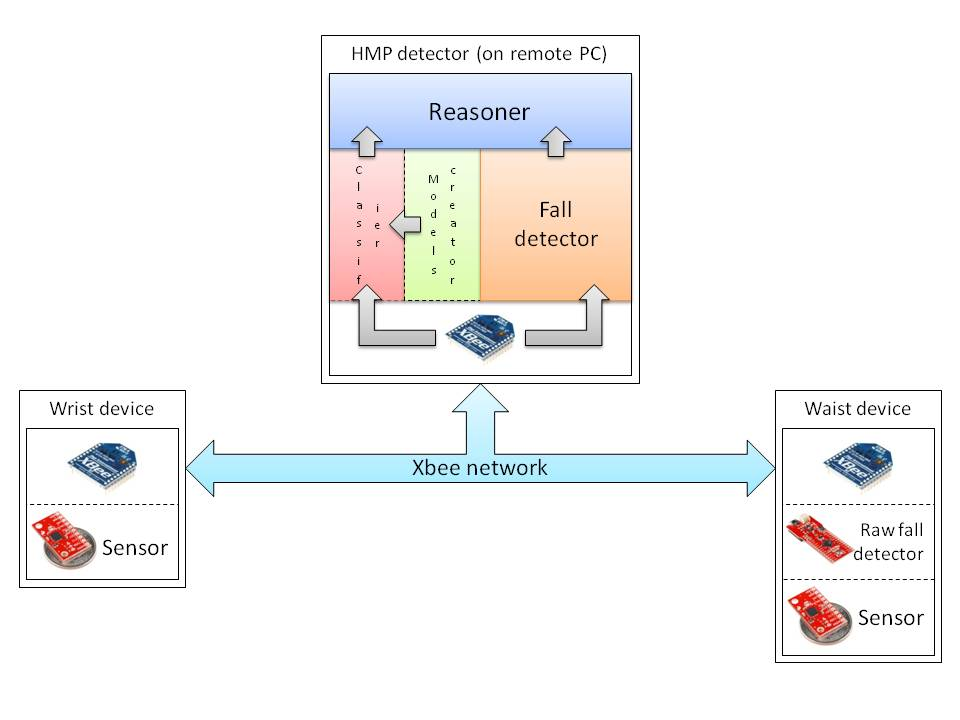
\includegraphics[scale=0.45]{system_architecture.jpg}
\caption{System architecture}
\end{figure}

HMPdetector provides a command-line interface for the Models Creator, Classifier, Fall detector and Reasoner modules.
More specifically:
\begin{itemize}
\item the \textbf{Models Creator} module builds the models of the considered human motion primitives by applying Gaussian Mixture Modelling and Gaussian Mixture Regression over a provided set of modelling trials (stored inside the motion-corresponding folder inside the Models folder);
\item the \textbf{Classifier} module performs (i) off-line analysis of recorded acceleration data (stored inside the Validation folder) and (ii) on-line analysis of acceleration data coming from the wrist device. It returns the possibility value of each motion primitive to be the one executed at each time instant;
\item the \textbf{Fall detector} module performs on-line acquisition of the fall alarm and related signals generated by the waist device in case a fall is detected and integrates them with wrist-motion information extracted from the acceleration data coming from the wrist device;
\item the \textbf{Reasoner} module performs (i) off-line and (ii) on-line analysis of the possibility values computed by the Classifier module and publishes the results as tuples in the PEIS tuple space under the key “activity”. It publishes the results of the fall detection performed by the Fall detector module as tuples under the key “fall”.
\end{itemize}

To access function-specific basic information and usage examples within the system, in a Terminal tab move to the HMP Detector extraction folder and type \verb+./HMPdetector -h+ or \verb+./HMPdetector--help+.

\section{Basic Human Motion Primitives}

HMPdetector comes with the training and validation dataset for $9$ basic Human Motion Primitives:
\begin{center}
\begin{tabular}{|c|p{6cm}|c|}
\hline
\textbf{Name} & \textbf{Description} & \textbf{Characteristics}\\
\hline
Climb & to climb 3 steps of a staircase & $\#$simple, $\#$recursive, $\#$full-body\\
\hline
GetUp & to get up from a lying position on a bed & $\#$simple, $\#$full-body\\
\hline
PickUpDrink & to pick up a glass from the table and start drinking from it & $\#$complex, $\#$hand-only\\
\hline
PickUpPour & to pick up a bottle from the table and start pouring its content in a glass on the table & $\#$complex, $\#$hand-only\\
\hline
PutDownDrink & to stop drinking from a glass and put it down on the table & $\#$complex, $\#$hand-only\\
\hline
PutDownDrink & to stop pouring the content of a bottle in a glass on the table and put it down on the table & $\#$complex, $\#$hand-only\\
\hline
Sit & to sit down on a chair & $\#$simple, $\#$full-body\\
\hline
Stand & to stand up from a chair & $\#$simple, $\#$full-body\\
\hline
Walk & to take 3 steps & $\#$simple, $\#$recursive, $\#$full-body\\
\hline
\end{tabular}
\end{center}

\chapter{Tutorials}

This and following tutorials assume that the HMPdetector executable file is located in folder: \verb+Documents/HMPdetector+.

This and following tutorials assume that the HMPdetector has been correctly installed and built, according to the procedure detailed in Section \ref{Installation Guide}.

\section{Display program help}
\begin{enumerate}
\item open a new Terminal tab
\item move inside the HMPdetector folder\\
(type \verb+cd Documents/HMPdetector+)
\item type \verb+./HMPdetector --help+\\
(or equivalently \verb+./HMPdetector -h+)
\end{enumerate}

\section{Create the models of the default modelling dataset}
Assumptions:
\begin{itemize}
\item the default modelling dataset is stored in folder: \verb+./Models/Ovada+.
\end{itemize}
Procedure:
\begin{enumerate}
\item open a new Terminal tab
\item move inside the HMPdetector folder\\
(type \verb+cd Documents/HMPdetector+)
\item type \verb+./HMPdetector --model+\\
(or equivalently \verb+./HMPdetector -m+)
\end{enumerate}

\section{Create the models of an existing modelling dataset}
\label{Create the models of an existing modelling dataset}
Assumptions:
\begin{itemize}
\item there exists a valid modelling dataset in folder: \verb+./Models/myDataset+.
\end{itemize}
Procedure:
\begin{enumerate}
\item open a new Terminal tab
\item move inside the HMPdetector folder\\
(type \verb+cd Documents/HMPdetector+)
\item type \verb+./HMPdetector --model myDataset+\\
(or equivalently \verb+./HMPdetector -m myDataset+)
\end{enumerate}

\section{Load a set of existing models with default loading options}
\label{Load a set of existing models with default loading options}
Assumptions:
\begin{itemize}
\item there exists a valid modelling dataset in folder: \verb+./Models/myDataset+;
\item the corresponding models have been created as detailed in Tutorial \ref{Create the models of an existing modelling dataset}.
\end{itemize}
Procedure:
\begin{enumerate}
\item open a new Terminal tab
\item move inside the HMPdetector folder\\
(type \verb+cd Documents/HMPdetector+)
\item type \verb+./HMPdetector --load myDataset+\\
(or equivalently \verb+./HMPdetector -l myDataset+)
\end{enumerate}

\section{Validate a loaded model with an existing set of validation trials}
Assumptions:
\begin{itemize}
\item there exists a valid modelling dataset in folder: \verb+./Models/myDataset+;
\item the corresponding models have been created as detailed in Tutorial \ref{Create the models of an existing modelling dataset};
\item the corresponding models have been loaded as detailed in Tutorial \ref{Load a set of existing models with default loading options};
\item there exists a valid validation dataset composed of \verb+[N]+ trials for the model \verb+[myHMP]+ in folder: \verb+./Validation/myDataset+.
\end{itemize}
Procedure:
\begin{enumerate}
\item open a new Terminal tab
\item move inside the HMPdetector folder\\
(type \verb+cd Documents/HMPdetector+)
\item type \verb+./HMPdetector --validate [myHMP] myDataset [N]+\\
(or equivalently \verb+./HMPdetector -v [myHMP] myDataset [N]+)
\end{enumerate}

\section{Perform off-line classification of an existing long recording}
Assumptions:
\begin{itemize}
\item there exists a valid modelling dataset in folder: \verb+./Models/myDataset+;
\item the corresponding models have been created as detailed in Tutorial \ref{Create the models of an existing modelling dataset};
\item the corresponding models have been loaded as detailed in Tutorial \ref{Load a set of existing models with default loading options};
\item there exists a valid recording \verb+ mylongTest.txt+ in folder: \verb+./Validation/longTest+.
\end{itemize}
Procedure:
\begin{enumerate}
\item open a new Terminal tab
\item move inside the HMPdetector folder\\
(type \verb+cd Documents/HMPdetector+)
\item type \verb+./HMPdetector --test mylongTest.txt+\\
(or equivalently \verb+./HMPdetector -t mylongTest.txt+)
\end{enumerate}

\chapter{Advanced Operations}
\section{Modify the modelling parameters of an existing modelling dataset}
Assumptions:
\begin{itemize}
\item there exists a valid modelling dataset in folder: \verb+./Models/myDataset+.
\end{itemize}

A valid modelling dataset contains a configuration file named \verb+HMPconfig.txt+, which defines:
\begin{itemize}
\item the HMP to be modelled, among the ones provided in the dataset;
\item the modelling parameters for each considered HMP.
\end{itemize}

Each line in the file \verb+HMPconfig.txt+ corresponds to one HMP to be modelled by the creator and is defined according to the following convention:
\begin{center}
[name] [nbMT] [nbGG] [nbBG]
\end{center}
where:
\begin{itemize}
\item \textbf{[name]} is the name of the HMP to be modelled by the creator, matching the name of the folder inside the dataset containing the modelling trials for the HMP;
\item \textbf{[nbMT]} is the number of modelling trials for the HMP;
\item \textbf{[nbGG]} is the number of Gaussian clusters that should be used by the creator to model the gravity feature of the HMP;
\item \textbf{[nbBG]} is the number of Gaussian clusters that should be used by the creator to model the body acceleration feature of the HMP.
\end{itemize}

By removing a line from the file \verb+HMPconfig.txt+ the corresponding HMP will not be modelled by the creator.

By adding/modifying a line of the file \verb+HMPconfig.txt+ the corresponding HMP will be modelled by the creator according to the specified parameters.

\section{Modify the classification parameters of an existing modelling dataset}
Assumptions:
\begin{itemize}
\item there exists a valid modelling dataset in folder: \verb+./Models/myDataset+.
\end{itemize}

A valid modelling dataset contains a configuration file named \verb+Classifierconfig.txt+, which defines:
\begin{itemize}
\item the HMP to be considered for classification, among the ones provided in the dataset;
\item the classification parameters for each considered HMP.
\end{itemize}

The first line in the file \verb+Classifierconfig.txt+ defines the total number of HMP to be considered for classification.

Each subsequent line corresponds to one HMP to be considered by the classifier and is defined according to the following convention:
\begin{center}
[name] [wG] [wB] [th]
\end{center}
where:
\begin{itemize}
\item \textbf{[name]} is the name of the HMP to be considered by the classifier, matching the name of the folder inside the dataset containing the modelling trials for the HMP;
\item \textbf{[wG]} is the weight of the gravity feature for the HMP (default: 0.5);
\item \textbf{[wB]} is the weight of the body acceleration feature for the HMP (default: 0.5);
\item \textbf{[th]} is the threshold on the distance to the model for a positive recognition of the HMP.
\end{itemize}

By removing a line from the file \verb+Classifierconfig.txt+ the corresponding HMP will not be considered by the classifier.

By adding/modifying a line of the file \verb+Classifierconfig.txt+ the corresponding HMP will be considered by the classifier and classification will be performed according to the specified parameters.

\end{document}
